\documentclass[30pt, a0paper, portrait, blockverticalspace=.5cm]{tikzposter}
\usepackage[utf8]{inputenc}
\usepackage{amssymb,amsfonts,amsmath,mathtext,mathtools}
\usepackage{xfrac}
\usepackage{enumitem}

\usepackage{makecell}
\usepackage{amsmath}

\let\vec\oldvec
\newcommand{\vec}[1]{\boldsymbol{#1}}

\title{\parbox{\linewidth}
	{\centering
		Dual-structure features for heavy ion and light particles at NICA collider
\\		
}}

\author{Kolokolchikov S.\textsuperscript{1*}, Senichev Yu.\textsuperscript{1}, Aksentyev A.,\textsuperscript{1,2}, Melnikov A. \textsuperscript{1,3}}
\institute{
	\textsuperscript{1} Institute for Nuclear Research of the Russian Academy of Sciences, Moscow, Russia\\
	\textsuperscript{2} National Research Nuclear University MEPhI, Moscow, Russia\\
	\textsuperscript{3} Landau Institute for Theoretical Physics, Chernogolovka, Russia\\
	*sergey.bell13@gmail.com
}
\usetheme{Simple}
\usecolorstyle{Russia}
\colorlet{blocktitlefgcolor}{black}

\usepackage{caption}
\captionsetup{font=large}
\usepackage{multicol}
\setlength\columnsep{1.5cm}

\begin{document}

\maketitle

\begin{columns}
\column{.33}

\block{Introduction}{

\par For successful collider experiments, it is essential to maintain a sufficient beam lifetime. Additionally, it is crucial to solve transition energy issue in order to achieve the desired beam emittance required for high luminosity. 
\par The dual magneto-optical structure opens up the prospect of accelerating both heavy ions, such as gold, and light particles like protons and deuterons.}

\block{Beam Lifetime}{

The lifetime of the beam luminosity in a collider experiment is achieved through the reduction of intra-beam scattering effects, coupled with the application of stochastic and electron beam cooling techniques. This approach assumes particular significance when dealing with high-intensity ion beams.

\begin{equation}
\begin{aligned}
& \frac{d \varepsilon}{d t}=\underbrace{-\frac{1}{\tau_{t r}} \cdot \varepsilon}_{\text {cooling }}+\underbrace{\left(\frac{d \varepsilon}{d t}\right)_{I B S}}_{\text {heating }} \\
& \frac{d \delta^2}{d t}=\underbrace{-\frac{1}{\tau_{\text {long }}} \cdot \delta^2}_{\text {cooling }}+\underbrace{\left(\frac{d \delta^2}{d t}\right)_{\text {IBS }}}_{\text {heating }} \\
&
\end{aligned}
\end{equation}

$\varepsilon$ – transverse emittance, $\tau_{tr}, \tau_{\mathrm{long\ }}$ – transverse/longitudinal cooling time, $\delta$ – momentum spread.
}

\block{Stochastic Cooling}{
\par The cooling rate can be determined [1]:

\begin{equation}
\frac{1}{\tau_{t r, l}}=\frac{W}{N}[\underbrace{2 g \cos \theta\left(1-1 / M_{p k}^2\right)}_{\begin{array}{c}
\text { coherent } \\
\text { effect(cooling) }
\end{array}}-\underbrace{g^2\left(M_{k p}+U\right)}_{\begin{array}{c}
\text { incoherent } \\
\text { effect(heating) }
\end{array}}]
\end{equation}

The mixing coefficients are defined as

\begin{equation}
\begin{aligned}
M_{p k} & =\frac{1}{2\left(f_{\max }+f_{\min }\right) \eta_{p k} T_{p k} \frac{\Delta p}{p}}, \\
M_{k p} & =\frac{1}{2\left(f_{\max }-f_{\min }\right) \eta_{k p} T_{k p} \frac{\Delta p}{p}}
\end{aligned}
\end{equation}

	\begin{minipage}{0.5\linewidth}
			\begin{tikzpicture}
			\node (cone) at (0,0) {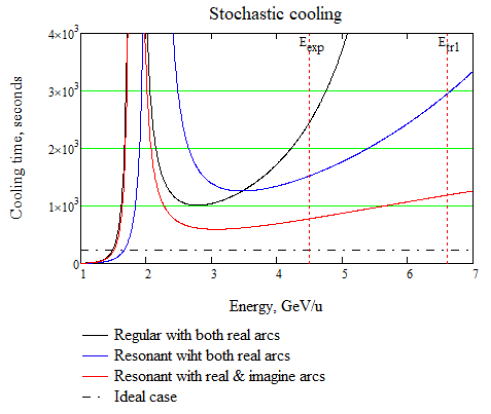
\includegraphics[width=\linewidth]{img/SC}};
			\end{tikzpicture}
		\end{minipage}
		\begin{minipage}{0.5\linewidth}
			\begin{tikzpicture}
			\node (cone) at (0,0) {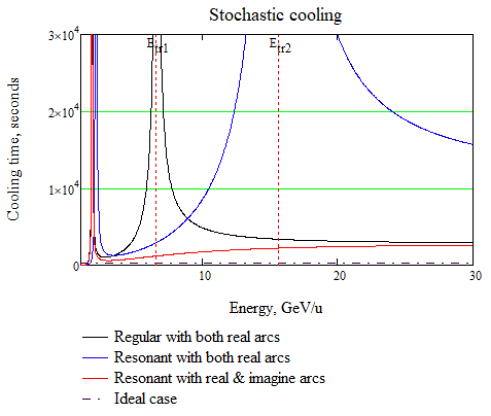
\includegraphics[width=\linewidth]{img/SC_wide}};
			\end{tikzpicture}
		\end{minipage}

}

\column{.33}

\block{Structures}{

	\begin{tikzpicture}
			\node (cone) at (0,0) {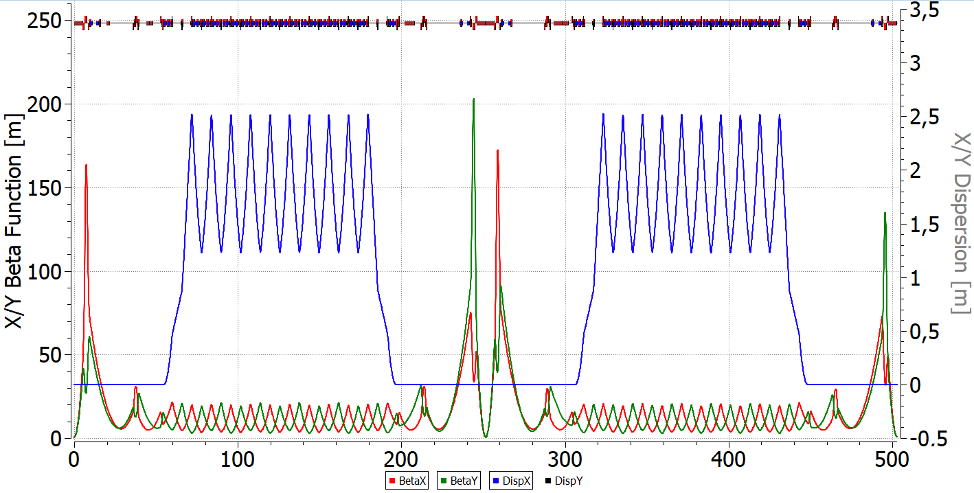
\includegraphics[width=\linewidth]{img/regular}};
	\end{tikzpicture}
 \textbf{"Regular".}	
	The straight sections remain constant in all structures. Their arrangement doesn't affect the IBS and transition energy. To suppress dispersion in the \textit{“regular”} structure used ‘missing magnets’ technic [2].
		
	
	\begin{tikzpicture}
			\node (cone) at (0,0) {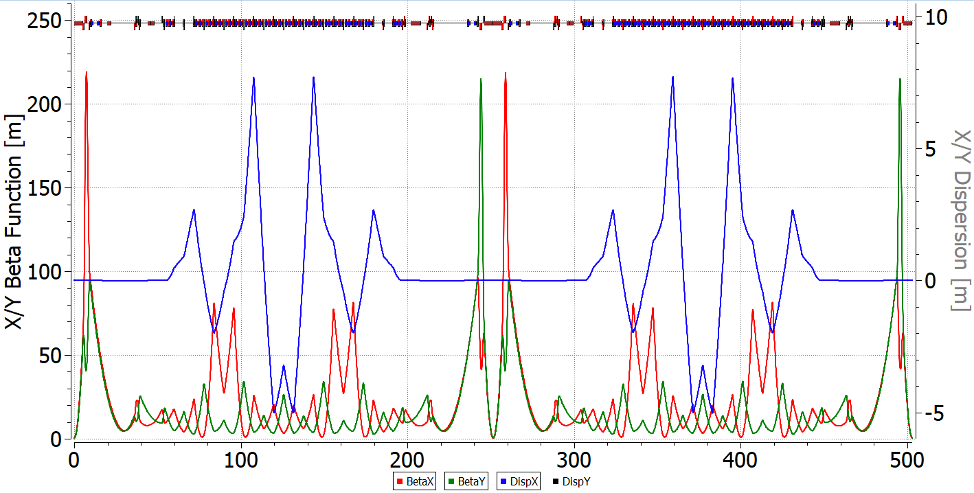
\includegraphics[width=\linewidth]{img/resonant}};
		\end{tikzpicture}
 \textbf{"Resonant".}		
		Based on the resonant principle [3] and can be obtained from \textit{"regular"} one by dividing quadrupoles into 2 families. Transition energy can be adjusted to increase it above the experiment energy.	

	\begin{tikzpicture}
			\node (cone) at (0,0) {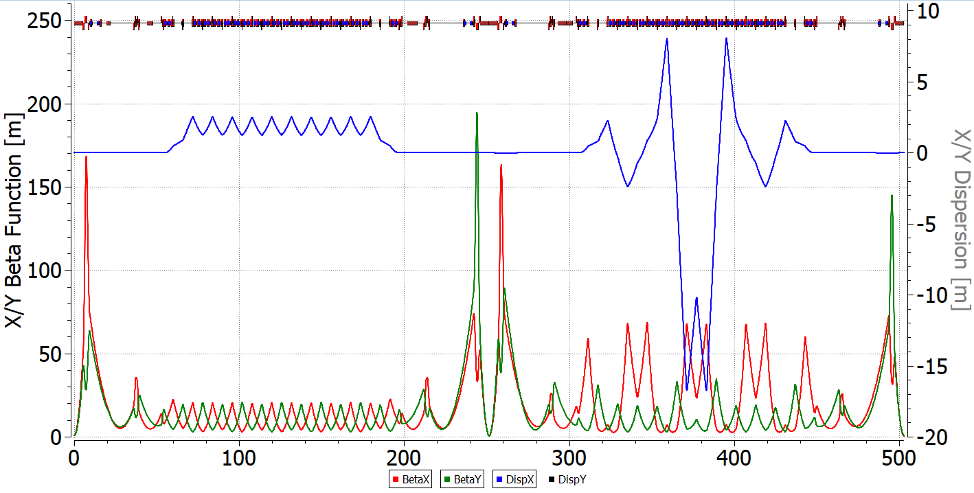
\includegraphics[width=\linewidth]{img/combined}};
		\end{tikzpicture}
	 \textbf{"Combined".}		
	In the case of a \textit{“combined”} structure, one arc operates in a \textit{regular} mode,
	\begin{equation}
\eta_{p k}=1 / \gamma_{t r}^2-1 / \gamma^2
\end{equation}
while the other employs resonant modulation 
\begin{equation}
\eta_{kp}=-1/\gamma_{tr}^2-1/\gamma^2\ \ \ 
\end{equation}
\newline
In \textit{"resonant"} optics the second asymptotic is at higher energy compared to the \textit{“regular”}. In \textit{“combined”}, the cooling efficiency is closer to the ideal value in a large energy range from 2.5 to 4.5 GeV, while in \textit{“regular”} optics the cooling rate is almost two times lower at the most optimal point $\sim3$ GeV. This behaviour is explained by absence of the second point of asymptotic growth.

}

\column{.33}
\block{Intra-Beam Scattering (IBS)}{

The selection of an appropriate cooling technique hinges on comparing its characteristic time scales with the rate at which the beam is heated due to intra-beam scattering.

\begin{equation}
\frac{1} {\tau_{I B S}}=\frac{\sqrt{\pi}}{4} \frac{c Z^2 r_p^2 L_C N}{A\cdot C_{\text {orb}}} \frac{\left\langle\beta_x\right\rangle}{\beta^3 \gamma^3 \varepsilon_x^{5 / 2}\left\langle\sqrt{\beta_x}\right\rangle}\left(\left\langle\frac{D_x^2+\dot{D}_x^2}{\beta_x^2}\right\rangle-\frac{1}{\gamma^2}\right)
\end{equation}

It should be expected that in optics with a value $\eta$ close to zero, the heating rate should decrease. Heavy ion beam ${_{79}^{197}}Au$ of the NICA collider with maximum luminosity ${10}^{27}\ {sm}^{-2}s^{-1}$.

	\begin{tikzpicture}
			\node (cone) at (0,0) {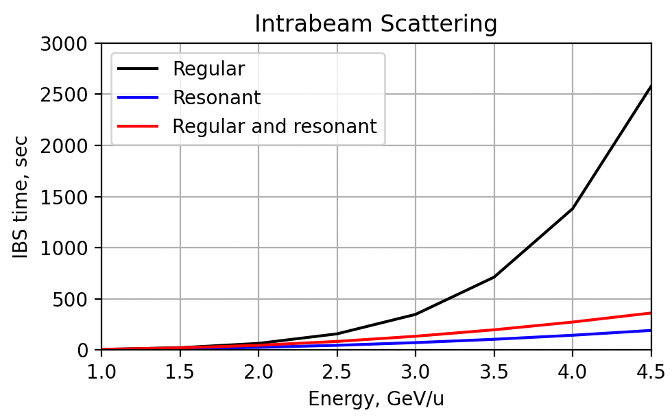
\includegraphics[width=\linewidth]{img/IBS}};
		\end{tikzpicture}
		
It can be concluded that in a \textit{regular} structure, stochastic cooling is able to balance intra-beam scattering in the energy range $W\geq4.5$ GeV. In \textit{resonant} structures, the IBS time is notably reduced. This is explained by the fact that the structure has a greater ratio $\left\langle\frac{D_x^2+{\dot{D}}_x^2}{\beta_x^2}\right\rangle$ between the dispersion and the beam $\beta$-function than in the case of a \textit{regular}. Thus, for the case of heavy ions, the configuration should be \textit{regular} and minimally modulated. Electron cooling is used in the \textit{regular} structure to cool the beam lower 4.5 GeV.		
}
\block{Transition Energy}{

In the context of light nuclei, such as protons and deuterons, the IBS time experiences a significant increase as the charge decreases. Consequently, the issue of intra-beam scattering becomes critical for heavy-ion beam.
	Owing to the charge-to-mass ratio, the peak energy of the proton beam amounts to approximately 13 GeV. Meanwhile, the transition energy of the \textit{“regular”} structure, which acts as a characteristic of the accelerator magneto-optical structure, stands at 5.7 GeV. Thus, transition energy needs to be overcome. Previously, has been demonstrated that dispersion modulation can increases transition energy or even reaches a complex value in a \textit{“resonant”} structure [4]. 

}


\end{columns}

\begin{columns}
\column{.5}

	\block{CONCLUSION}{
\par The dual magneto-optical structure is proposed for accelerating both heavy ion and light particle beams, exemplified by the NICA facility. Shown that the stochastic cooling time in \textit{“resonant”} and \textit{“combined”} structures is significantly shorter than in \textit{“regular”} ones. However, due to modulation of $\beta$-function and D dispersion, the time of intra-beam scattering decreases. For this reason, a \textit{“regular”} magneto-optic structure with minimally modulated dispersion and $\beta$-function is optimal in the heavy-ion mode. In the case of protons, the problem of overcoming the transition energy is important, for this a \textit{“resonant”} or \textit{“combined”} magneto-optical structure can be used. It does not require a significant adjustment, only the allocation of a separate focusing quadrupole family.
}

\column{.5}
	\block{REFERENCES}{
	 
	\par [1] D. Möhl, G. Petrucci, L. Thorndahl and S. van der Meer, Phys. Rep. 58 (1980) 75 
	\par [2]  Grigory Trubnikov, Anatoly Sidorin, Nikolay Shurkhno, NICA cooling program, CYBERNETICS AND PHYSICS, Vol. 3, No. 3. 2014, 137-146
	\par [3] Senichev, Y.V., Chechenin, A.N. Theory of “Resonant” lattices for synchrotrons with negative momentum compaction factor. J. Exp. Theor. Phys. 105, 988–997 (2007). https://doi.org/10.1134/S1063776107110118
	\par [4] Kolokolchikov, S.D., Senichev, Y.V. Magneto-Optical Structure of the NICA Collider with High Transition Energy. Phys. Atom. Nuclei 84, 1734–1742 (2021). https://doi.org/10.1134/S1063778821100185
	}
	
\end{columns}

\end{document}